\documentclass[11pt,a4paper]{article}
\usepackage[utf8]{inputenc}
\usepackage[T1]{fontenc}
\usepackage[portuguese]{babel}
\usepackage{amsmath, amssymb, graphicx, float, setspace, hyperref}
\usepackage[top=1.5cm,bottom=1.5cm,left=1.75cm,right=1.75cm]{geometry}
\usepackage[tiny]{titlesec} 
\usepackage{parskip, booktabs, array}
\usepackage{listings, tabularx}

\hypersetup{colorlinks=true, allcolors=blue}

\begin{document}
\onehalfspacing
\begin{center}
    \vspace*{0.5cm}
    {\LARGE \textbf{Trabalho 03: Sistema de Matchmaking}} \\
    \textit{Estrutura de Dados} \\
    \vspace{0.8cm}

    \begin{minipage}{0.45\textwidth}
        \centering
        \textbf{Rafael Gontijo Ferreira} \\
        \href{mailto:rafael.ferreira.2@fgv.edu.br}{\footnotesize \texttt{rafael.ferreira.2@fgv.edu.br}}
    \end{minipage}
    \begin{minipage}{0.45\textwidth}
        \centering
        \textbf{Rudá Dantas Ruoso Brandão} \\
        \href{mailto:rudabrandao@ruoso.com}{\footnotesize \texttt{rudabrandao@ruoso.com}}
    \end{minipage}
    
    \vspace{0.8cm}
\end{center}

\section{Descrição do Projeto}
 
Este trabalho apresenta a implementação de um sistema de \textit{matchmaking} para jogadores online, desenvolvido como terceira atividade de Estrutura de Dados. O objetivo central é gerenciar uma fila de espera de jogadores e formar grupos com níveis de habilidade próximos, explorando algoritmos de ordenação como ferramenta central para tornar essa busca eficiente.
 
O sistema suporta as seguintes operações fundamentais:
 
\begin{itemize}
    \item \textbf{Inserção:} Adiciona um jogador ao final da fila de espera.
    \item \textbf{Remoção:} Remove um jogador da fila de espera  pelo seu identificador único.
    \item \textbf{Recuperação:} Recuperação de uma cópia da lista de espera atual.
    \item \textbf{Exibição:} Exibição da fila de espera atual.
    \item \textbf{Ordenação:} Ordena a fila por score crescente; desempate por timestamp.
    \item \textbf{Formação de grupo:} Retorna o primeiro grupo válido de jogadores consecutivos na fila ordenada.
\end{itemize}
 
\section{Organização do Sistema}
 
O projeto é modularizado nos seguintes arquivos:
 
\begin{itemize}
    \item \texttt{main.cpp}: Ponto de entrada com testes funcionais e benchmark de desempenho.
    \item \texttt{Player} (\texttt{.hpp}/\texttt{.cpp}): Declaração e implementação da classe \texttt{Player}
    \item \texttt{Matchmaking} (\texttt{.hpp}/\texttt{.cpp}): Declaração e implementação da classe \texttt{Matchmaking}.
    \item \texttt{grafico.ipynb}: Notebook Python para geração dos gráficos de desempenho com os dados de benchmark.
\end{itemize}


O projeto compila com:
 
\begin{lstlisting}
g++ main.cpp Matchmaking.cpp Player.cpp -o matchmaking
\end{lstlisting}
 
\section{Estruturas de Dados e Implementação}

\subsection{Array Dinâmico}
 
A classe \texttt{Matchmaking} armazena os jogadores em um array alocado dinamicamente no construtor com capacidade \texttt{MAX\_PLAYERS}, e liberado no destrutor:
 
\begin{lstlisting}[language=C++]
players = new Player[MAX_PLAYERS];  // construtor
delete[] players;                   // destrutor
\end{lstlisting}
 
Essa abordagem evita o risco de estouro de pilha que ocorreria com um array estático de 100.000 elementos do tipo \texttt{Player} declarado diretamente no corpo da classe.

 \subsection{Inserção e Remoção}
 
A \textbf{inserção} coloca o novo jogador ao final do array e incrementa o contador de tamanho, sendo uma operação $O(1)$. A \textbf{remoção} por ID percorre o array linearmente e, ao encontrar o elemento, desloca todos os subsequentes uma posição para a esquerda, compactando o array, tendo custo $O(n)$. Essa compactação é necessária para não corromper a lista e permitir o funcionamento da lógica de remoção de grupos.

\section{Algoritmos de Ordenação}
 
Ambos os algoritmos ordenam os jogadores por score crescente e, em caso de empate, por
timestamp crescente. Nenhuma função de ordenação da STL foi utilizada.
 
\subsection{Insertion Sort}
 
O \textit{Insertion Sort} mantém um prefixo ordenado do array. A cada iteração $i$, o elemento na posição $i$ é inserido na posição correta dentro do prefixo $[0, i-1]$ por meio de trocas sucessivas com seu vizinho esquerdo, interrompidas quando a condição de ordem é satisfeita. Em caso de empate de score, é avaliado o timestamp de cada jogador.
 
\textbf{Custo:} $O(n^2)$ no pior caso e, para arrays quase ordenados, $O(n \cdot k)$, onde $k$ representa a distância máxima entre um jogador e sua posição correta.

\subsection{Merge Sort}
 
O \textit{Merge Sort} é implementado recursivamente por uma função auxiliar \texttt{sortByScoreMerge(low\_bound, up\_bound)}. A cada chamada, o segmento é dividido ao meio, cada metade é ordenada recursivamente, e os dois segmentos são intercalados em um array auxiliar alocado dinamicamente, copiado de volta ao array principal e então liberado. Novamente, a intercalação aplica os dois critérios de comparação: score e, em empate, timestamp.
 
\textbf{Custo:} $O(n \log n)$ em todos os casos. A cada nível da árvore de recursão é realizada a intercalação sobre o array completo (dividido em vários segmentos), o que tem custo $O(n)$. O processo de divisão gera $O(\log n)$ níveis. 

\section{Formação de Grupos}
 
O método \texttt{formGroup(groupSize, delta, n)} assume uma ordenação prévia dos jogadores. Dado que o array está ordenado por score, em qualquer janela contígua de \texttt{groupSize} elementos o menor score está na primeira posição e o maior na última. Portanto, basta verificar a diferença de score entre o primeiro e último jogador da janela:
 
\begin{lstlisting}[language=C++]
players[i + groupSize - 1].getScore() - players[i].getScore() <= delta
\end{lstlisting}
 
O método percorre o array com uma \textbf{janela deslizante} de tamanho \texttt{groupSize}, testando cada posição inicial $i$. Ao encontrar a primeira janela válida, copia os jogadores para um novo array alocado dinamicamente e os remove da fila via \texttt{removePlayer}. A liberação do ponteiro retornado fica a cargo de quem chama a função.
 
Sem a ordenação prévia, seria necessário testar todas as combinações de $g$ elementos, tendo um custo $O(n^g)$. Com a ordenação, a busca pela janela é $O(n)$ e as remoções custam $O(g \cdot n)$, resultando em custo total $O(n \log n + g \cdot n)$ para uma ordenação via \textit{Merge Sort}.

\section{Custo Computacional}
 
\begin{center}
\begin{tabular}{L{4.2cm} C{2.8cm} L{6.5cm}}
  \toprule
  \textbf{Operação} & \textbf{Complexidade} & \textbf{Observação} \\
  \midrule
  Inserção               & $O(1)$              & Inserção ao final do array. \\
  Remoção por ID         & $O(n)$              & Busca linear + compactação. \\
  Insertion Sort         & $O(n^2)$ / $O(n)$   & Pior / melhor caso. \\
  Merge Sort             & $O(n \log n)$       & Todos os casos. \\
  Formação de grupo      & $O(n + g \cdot n)$  & Busca $O(n)$ + remoções $O(g \cdot n)$. \\
  \texttt{getWaitingPlayers} & $O(n)$          & Cópia integral do array interno. \\
  \bottomrule
\end{tabular}

\small Tabela 1: Custo teórico para as funções implementadas
\end{center}

\section{Análise Experimental: Insertion Sort vs. Merge Sort}
 
\subsection{Metodologia}

Foram realizadas 10 amostras de teste, qm que, para cada uma foram geradas aleatórias por meio de \texttt{std::mt19937} com \textit{seed} variável (\texttt{std::random\_device}), com tamanho inicial \texttt{MAX\_PLAYERS} (100.000) reduzido geométricamente por um fator $2/3$ a cada iteração até $n=1$. Dentro de cada iteração de teste, as funções de \textit{Insertion} e \textit{Merge Sort} foram avaliadas com a mesma entrada aleatória. Os resultados foram armazenados em \texttt{out.csv} e analizados em \texttt{python} via \texttt{seaborn} e \texttt{pandas}
 
\subsection{Resultados}
 
\begin{center}
\begin{tabular}{R{2.8cm} R{3.2cm} R{3.2cm} R{2.4cm}}
  \toprule
  \textbf{$n$ (jogadores)} & \textbf{Insertion Sort (s)} & \textbf{Merge Sort (s)} & \textbf{Razão} \\
  \midrule
  100.000 & $\approx 104{,}7$    & $\approx 0{,}15$  & ${\sim}698\times$ \\
   66.666 & $\approx 47{,}3$    & $\approx 0{,}095$  & ${\sim}497\times$ \\
   44.444 & $\approx 20{,}0$    & $\approx 0{,}060$  & ${\sim}333\times$ \\
   29.629 & $\approx 9{,}0$     & $\approx 0{,}038$  & ${\sim}236\times$ \\
   19.752 & $\approx 4{,}0$     & $\approx 0{,}025$  & ${\sim}160\times$ \\
   13.168 & $\approx 1{,}7$     & $\approx 0{,}016$  & ${\sim}106\times$ \\
    8.778 & $\approx 0{,}77$    & $\approx 0{,}010$  & ${\sim}77\times$  \\
    5.852 & $\approx 0{,}34$    & $\approx 0{,}0065$  & ${\sim}52\times$  \\
    3.901 & $\approx 0{,}15$    & $\approx 0{,}0041$  & ${\sim}36\times$  \\
    2.600 & $\approx 0{,}067$   & $\approx 0{,}0027$  & ${\sim}24\times$  \\
    1.733 & $\approx 0{,}029$   & $\approx 0{,}0018$  &
    ${\sim}16\times$ \\
    1.155 & $\approx 0{,}011$   & $\approx 0{,}0011$  & ${\sim}10\times$  \\
     770 & $\approx 0{,}0054$   & $\approx 0{,}00072$ &
     ${\sim}7\times$ \\
     513 & $\approx 0{,}0025$  & $\approx 0{,}00045$ & ${\sim}5\times$   \\
  \bottomrule
\end{tabular}
 
\small Tabela 2: Tempos médios observados (10 amostras, entradas aleatórias).
\end{center}
 
\subsection{Discussão}
 
Os resultados são consistentes com as complexidades teóricas. Para $n = 100.000$, o \textit{Insertion Sort} levou cerca de 104,7~s, enquanto o \textit{Merge Sort} completou o mesmo trabalho em aproximadamente 0,15~s, uma diferença de quse 700 vezes. Essa razão cresce com $n$, o que é esperado: a diferença entre $O(n^2)$ e $O(n \log n)$ é amplificada à medida que
$n$ aumenta. 

\begin{figure}[H]
    \centering
    \begin{minipage}{0.7\textwidth}
        \centering
        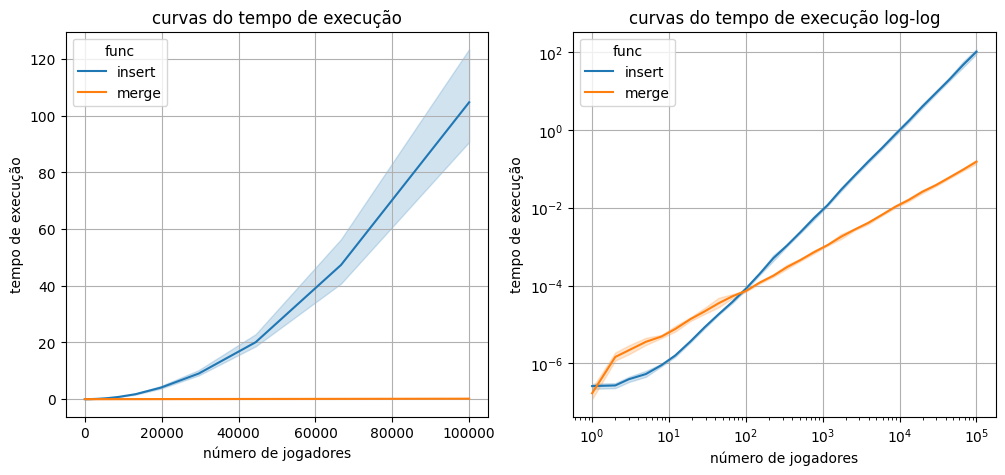
\includegraphics[width=\textwidth]{figs/Fig01.png}
        \caption{\small Curvas de tempo de execução}
        \label{fig1}
    \end{minipage}
    \hfill
\end{figure}
 
Nos gráficos em escala log-log, as curvas do Insertion Sort e do Merge Sort apresentam inclinações aproximadas de 2 e 1 (Figura \ref{fig1}), respectivamente, confirmando visualmente as complexidades teóricas. Para entradas pequenas ($n < 100$), a diferença absoluta de tempo é negligenciável apesar do \textit{overhead} de recursão e alocação auxiliar do Merge Sort ser desfavorável.

\begin{figure}[H]
    \centering
    \begin{minipage}{0.7\textwidth}
        \centering
        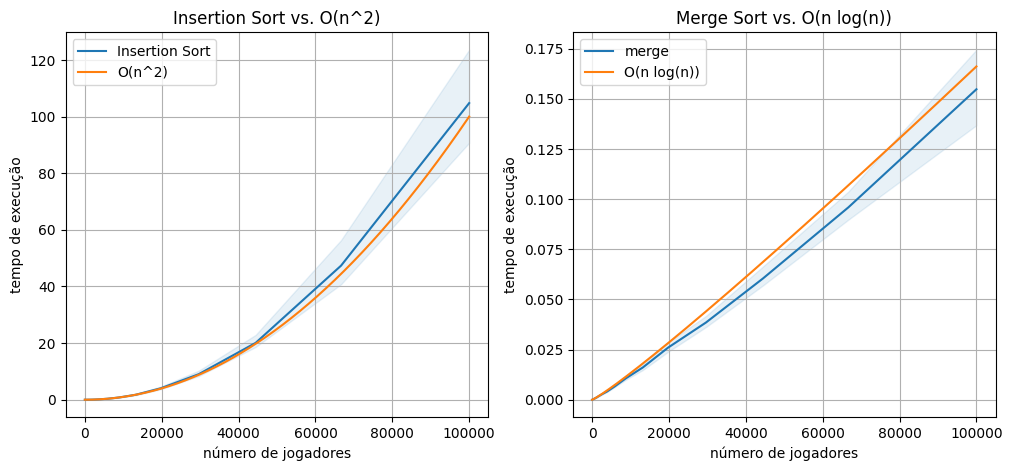
\includegraphics[width=\textwidth]{figs/Fig02.png}
        \caption{\small Custo medido x teórico}
        \label{fig2}
    \end{minipage}
    \hfill
\end{figure}

Além disso, comparando o desempenho das funções com a curva de suas complexidades teóricas, podemos reafirmar esse dado (Figura \ref{fig2}).
 
Em síntese, o Merge Sort é amplamente superior para filas de espera com muitos jogadores. O Insertion Sort tem relevância apenas como referência de implementação simples ou para listas já quase ordenadas, onde seu custo se aproxima de $O(n)$.
 
\end{document}
 
